% Options for packages loaded elsewhere
\PassOptionsToPackage{unicode}{hyperref}
\PassOptionsToPackage{hyphens}{url}
%
\documentclass[
]{article}
\usepackage{lmodern}
\usepackage{amssymb,amsmath}
\usepackage{ifxetex,ifluatex}
\ifnum 0\ifxetex 1\fi\ifluatex 1\fi=0 % if pdftex
  \usepackage[T1]{fontenc}
  \usepackage[utf8]{inputenc}
  \usepackage{textcomp} % provide euro and other symbols
\else % if luatex or xetex
  \usepackage{unicode-math}
  \defaultfontfeatures{Scale=MatchLowercase}
  \defaultfontfeatures[\rmfamily]{Ligatures=TeX,Scale=1}
\fi
% Use upquote if available, for straight quotes in verbatim environments
\IfFileExists{upquote.sty}{\usepackage{upquote}}{}
\IfFileExists{microtype.sty}{% use microtype if available
  \usepackage[]{microtype}
  \UseMicrotypeSet[protrusion]{basicmath} % disable protrusion for tt fonts
}{}
\makeatletter
\@ifundefined{KOMAClassName}{% if non-KOMA class
  \IfFileExists{parskip.sty}{%
    \usepackage{parskip}
  }{% else
    \setlength{\parindent}{0pt}
    \setlength{\parskip}{6pt plus 2pt minus 1pt}}
}{% if KOMA class
  \KOMAoptions{parskip=half}}
\makeatother
\usepackage{xcolor}
\IfFileExists{xurl.sty}{\usepackage{xurl}}{} % add URL line breaks if available
\IfFileExists{bookmark.sty}{\usepackage{bookmark}}{\usepackage{hyperref}}
\hypersetup{
  hidelinks,
  pdfcreator={LaTeX via pandoc}}
\urlstyle{same} % disable monospaced font for URLs
\usepackage{color}
\usepackage{fancyvrb}
\newcommand{\VerbBar}{|}
\newcommand{\VERB}{\Verb[commandchars=\\\{\}]}
\DefineVerbatimEnvironment{Highlighting}{Verbatim}{commandchars=\\\{\}}
% Add ',fontsize=\small' for more characters per line
\newenvironment{Shaded}{}{}
\newcommand{\AlertTok}[1]{\textcolor[rgb]{1.00,0.00,0.00}{\textbf{#1}}}
\newcommand{\AnnotationTok}[1]{\textcolor[rgb]{0.38,0.63,0.69}{\textbf{\textit{#1}}}}
\newcommand{\AttributeTok}[1]{\textcolor[rgb]{0.49,0.56,0.16}{#1}}
\newcommand{\BaseNTok}[1]{\textcolor[rgb]{0.25,0.63,0.44}{#1}}
\newcommand{\BuiltInTok}[1]{#1}
\newcommand{\CharTok}[1]{\textcolor[rgb]{0.25,0.44,0.63}{#1}}
\newcommand{\CommentTok}[1]{\textcolor[rgb]{0.38,0.63,0.69}{\textit{#1}}}
\newcommand{\CommentVarTok}[1]{\textcolor[rgb]{0.38,0.63,0.69}{\textbf{\textit{#1}}}}
\newcommand{\ConstantTok}[1]{\textcolor[rgb]{0.53,0.00,0.00}{#1}}
\newcommand{\ControlFlowTok}[1]{\textcolor[rgb]{0.00,0.44,0.13}{\textbf{#1}}}
\newcommand{\DataTypeTok}[1]{\textcolor[rgb]{0.56,0.13,0.00}{#1}}
\newcommand{\DecValTok}[1]{\textcolor[rgb]{0.25,0.63,0.44}{#1}}
\newcommand{\DocumentationTok}[1]{\textcolor[rgb]{0.73,0.13,0.13}{\textit{#1}}}
\newcommand{\ErrorTok}[1]{\textcolor[rgb]{1.00,0.00,0.00}{\textbf{#1}}}
\newcommand{\ExtensionTok}[1]{#1}
\newcommand{\FloatTok}[1]{\textcolor[rgb]{0.25,0.63,0.44}{#1}}
\newcommand{\FunctionTok}[1]{\textcolor[rgb]{0.02,0.16,0.49}{#1}}
\newcommand{\ImportTok}[1]{#1}
\newcommand{\InformationTok}[1]{\textcolor[rgb]{0.38,0.63,0.69}{\textbf{\textit{#1}}}}
\newcommand{\KeywordTok}[1]{\textcolor[rgb]{0.00,0.44,0.13}{\textbf{#1}}}
\newcommand{\NormalTok}[1]{#1}
\newcommand{\OperatorTok}[1]{\textcolor[rgb]{0.40,0.40,0.40}{#1}}
\newcommand{\OtherTok}[1]{\textcolor[rgb]{0.00,0.44,0.13}{#1}}
\newcommand{\PreprocessorTok}[1]{\textcolor[rgb]{0.74,0.48,0.00}{#1}}
\newcommand{\RegionMarkerTok}[1]{#1}
\newcommand{\SpecialCharTok}[1]{\textcolor[rgb]{0.25,0.44,0.63}{#1}}
\newcommand{\SpecialStringTok}[1]{\textcolor[rgb]{0.73,0.40,0.53}{#1}}
\newcommand{\StringTok}[1]{\textcolor[rgb]{0.25,0.44,0.63}{#1}}
\newcommand{\VariableTok}[1]{\textcolor[rgb]{0.10,0.09,0.49}{#1}}
\newcommand{\VerbatimStringTok}[1]{\textcolor[rgb]{0.25,0.44,0.63}{#1}}
\newcommand{\WarningTok}[1]{\textcolor[rgb]{0.38,0.63,0.69}{\textbf{\textit{#1}}}}
\usepackage{graphicx}
\makeatletter
\def\maxwidth{\ifdim\Gin@nat@width>\linewidth\linewidth\else\Gin@nat@width\fi}
\def\maxheight{\ifdim\Gin@nat@height>\textheight\textheight\else\Gin@nat@height\fi}
\makeatother
% Scale images if necessary, so that they will not overflow the page
% margins by default, and it is still possible to overwrite the defaults
% using explicit options in \includegraphics[width, height, ...]{}
\setkeys{Gin}{width=\maxwidth,height=\maxheight,keepaspectratio}
% Set default figure placement to htbp
\makeatletter
\def\fps@figure{htbp}
\makeatother
\setlength{\emergencystretch}{3em} % prevent overfull lines
\providecommand{\tightlist}{%
  \setlength{\itemsep}{0pt}\setlength{\parskip}{0pt}}
\setcounter{secnumdepth}{-\maxdimen} % remove section numbering

\author{}
\date{}

\begin{document}

\hypertarget{ux5b9eux9a8cux76eeux6807}{%
\subsection{实验目标}\label{ux5b9eux9a8cux76eeux6807}}

使用数据集,网址:\url{http://www.cs.cmu.edu/afs/cs/project/theo-11/www/naive-bayes.html}

包含两个文本数据集:

\begin{enumerate}
\def\labelenumi{\arabic{enumi}.}
\item
  总数据集'20\_newsgroups':包含20种不同的新闻类别,总计共有19997篇文档,每种类别下应该平均有1000份新闻文档.
\item
  子类文档'mini\_newsgroups':由第一个总数据集中每种类别的新闻中随机选择100份,总计2000份文档,用于验证算法的准确度.
\end{enumerate}

使用第一个数据集对模型进行训练,用第二个数据集计算模型的准确率.

\hypertarget{ux5b9eux9a8cux73afux5883}{%
\subsection{实验环境}\label{ux5b9eux9a8cux73afux5883}}

\begin{verbatim}
Python		'3.9.12'
numpy		'1.20.0'
matplotlib	'3.5.1'
nltk		'3.7'
tensorflow	'2.6.0'
\end{verbatim}

编辑器为Jupyter notebook.
全部代码已上传至\href{https://github.com/wty-yy/LaTex-Projects/blob/main/NLP/hw2/code/main.ipynb}{GitHub}.

\hypertarget{ux6570ux636eux9884ux5904ux7406}{%
\subsection{数据预处理}\label{ux6570ux636eux9884ux5904ux7406}}

\hypertarget{ux6587ux4ef6ux8bfbux5165ux5904ux7406}{%
\subsubsection{文件读入处理}\label{ux6587ux4ef6ux8bfbux5165ux5904ux7406}}

将20种文件类型进行编号,并查看内部的文档数目,使用Python3.6以上的路径处理包
\texttt{pathlib} 中 \texttt{Path} 类,对文件路径进行处理:

\begin{Shaded}
\begin{Highlighting}[]
\KeywordTok{def}\NormalTok{ initDataset(fname, showInfo}\OperatorTok{=}\VariableTok{True}\NormalTok{):}
\NormalTok{    path }\OperatorTok{=}\NormalTok{ Path(fname)  }\CommentTok{\# 将路径转化为Path类}
\NormalTok{    folds }\OperatorTok{=}\NormalTok{ [f.name }\ControlFlowTok{for}\NormalTok{ f }\KeywordTok{in}\NormalTok{ path.iterdir() }\ControlFlowTok{if}\NormalTok{ f.is\_dir()]  }\CommentTok{\# 获取文件夹名称}
    \ControlFlowTok{for} \BuiltInTok{id}\NormalTok{, fold }\KeywordTok{in} \BuiltInTok{enumerate}\NormalTok{(folds):  }\CommentTok{\# 一共有20个文件夹,分别对其内部文件进行处理}
        \BuiltInTok{print}\NormalTok{(}\SpecialStringTok{f\textquotesingle{}处理第}\SpecialCharTok{\{}\BuiltInTok{id}\OperatorTok{+}\DecValTok{1}\SpecialCharTok{\}}\SpecialStringTok{/}\SpecialCharTok{\{}\BuiltInTok{len}\NormalTok{(folds)}\SpecialCharTok{\}}\SpecialStringTok{个文件夹}\SpecialCharTok{\{}\NormalTok{fold}\SpecialCharTok{\}}\SpecialStringTok{中...\textquotesingle{}}\NormalTok{)}
\NormalTok{        now }\OperatorTok{=}\NormalTok{ path.joinpath(fold)}
\NormalTok{        files }\OperatorTok{=}\NormalTok{ [f.name }\ControlFlowTok{for}\NormalTok{ f }\KeywordTok{in}\NormalTok{ now.iterdir() }\ControlFlowTok{if}\NormalTok{ f.is\_file()]  }\CommentTok{\# 获取当前文件夹内的文件名}
        \ControlFlowTok{for} \BuiltInTok{file} \KeywordTok{in}\NormalTok{ tqdm(files):  }\CommentTok{\# 获取文件文件名}
\NormalTok{            pathFile }\OperatorTok{=}\NormalTok{ now.joinpath(}\BuiltInTok{file}\NormalTok{)}
            \ControlFlowTok{with} \BuiltInTok{open}\NormalTok{(pathFile, errors}\OperatorTok{=}\StringTok{\textquotesingle{}replace\textquotesingle{}}\NormalTok{) }\ImportTok{as}\NormalTok{ f:  }\CommentTok{\# 打开文件进行处理}
       		\CommentTok{\#... 文档处理}
\end{Highlighting}
\end{Shaded}

通过观察文档内容,可以发现,文档主要是由两部分构成,第一部分为文档的相关信息,而正文与相关信息之间由一个换行符分开,所以我们通过判断第一个换行符,来提取正文部分.

\begin{verbatim}
Xref: ...
Newsgroups: ...
Path: ...
From: ...
Subject: ...
Message-ID: ...
Organization: ...
References: ...
Lines: ...

In article <C51C4r.BtG@csc.ti.com> rowlands@hc.ti.com (Jon Rowlands) writes:
... 以下都是正文
\end{verbatim}

\begin{Shaded}
\begin{Highlighting}[]
\ControlFlowTok{with} \BuiltInTok{open}\NormalTok{(pathFile, errors}\OperatorTok{=}\StringTok{\textquotesingle{}replace\textquotesingle{}}\NormalTok{) }\ImportTok{as}\NormalTok{ f:  }\CommentTok{\# 打开文件进行处理}
\NormalTok{    s }\OperatorTok{=}\NormalTok{ f.readline()}
    \ControlFlowTok{while}\NormalTok{ s }\OperatorTok{!=} \StringTok{"}\CharTok{\textbackslash{}n}\StringTok{"}\NormalTok{:  }\CommentTok{\# 先找到第一个换行符,下面则是正文}
\NormalTok{        s }\OperatorTok{=}\NormalTok{ f.readline()}
\NormalTok{        text }\OperatorTok{=}\NormalTok{ f.read()}
\end{Highlighting}
\end{Shaded}

\hypertarget{ux5206ux8bcdux64cdux4f5c}{%
\subsubsection{分词操作}\label{ux5206ux8bcdux64cdux4f5c}}

首先将20类的文档全部读入,将数据的主要成分提取出来,然后利用NLTK库的分词功能

\begin{enumerate}
\def\labelenumi{\arabic{enumi}.}
\item
  将文章转化为小写 \texttt{words.lower()}
\item
  划分 \texttt{nltk.word\_tokenize(words)}
\item
  标点符号去除,用正则表达式判断单词中是否包含英文,若不包含则删去
\item
  去除停用词,利用
  \texttt{nltk.corpus.stopwords(\textquotesingle{}english\textquotesingle{})}
  获得停用词词库
\item
  词干提取,使用 \texttt{nltk.stem.porter.PorterStemmer(word)}
  词干提取方法
\item
  词性还原,使用 \texttt{nltk.stem.WordNetLemmatizer(word)} 还原词性
\end{enumerate}

\begin{Shaded}
\begin{Highlighting}[]
\KeywordTok{def}\NormalTok{ extractWords(words):  }\CommentTok{\# 提取分词}
\NormalTok{    words }\OperatorTok{=}\NormalTok{ words.lower()}
\NormalTok{    words }\OperatorTok{=}\NormalTok{ word\_tokenize(words)  }\CommentTok{\# 分词}
\NormalTok{    dropWords }\OperatorTok{=}\NormalTok{ [}\StringTok{"n\textquotesingle{}t"}\NormalTok{]  }\CommentTok{\# 这个是计算结果中出现次数第一的,但明显不重要}
\NormalTok{    words }\OperatorTok{=}\NormalTok{ [word }\ControlFlowTok{for}\NormalTok{ word }\KeywordTok{in}\NormalTok{ words }\ControlFlowTok{if}\NormalTok{ re.match(}\VerbatimStringTok{r\textquotesingle{}[A{-}Za{-}z]\textquotesingle{}}\NormalTok{, word) }\KeywordTok{and}\NormalTok{ word }\KeywordTok{not} \KeywordTok{in}\NormalTok{ dropWords]  }\CommentTok{\# 保证单词中必须包含字母}
\NormalTok{    stops }\OperatorTok{=} \BuiltInTok{set}\NormalTok{(stopwords.words(}\StringTok{\textquotesingle{}english\textquotesingle{}}\NormalTok{))}
\NormalTok{    words }\OperatorTok{=}\NormalTok{ [word }\ControlFlowTok{for}\NormalTok{ word }\KeywordTok{in}\NormalTok{ words }\ControlFlowTok{if}\NormalTok{ word }\KeywordTok{not} \KeywordTok{in}\NormalTok{ stops]}
\NormalTok{    tmp }\OperatorTok{=}\NormalTok{ []  }\CommentTok{\# 词干提取+还原词性}
    \ControlFlowTok{for}\NormalTok{ word }\KeywordTok{in}\NormalTok{ words:}
\NormalTok{        stem }\OperatorTok{=}\NormalTok{ PorterStemmer().stem(word)  }\CommentTok{\# 词干提取}
\NormalTok{        pos }\OperatorTok{=}\NormalTok{ [}\StringTok{\textquotesingle{}n\textquotesingle{}}\NormalTok{, }\StringTok{\textquotesingle{}v\textquotesingle{}}\NormalTok{, }\StringTok{\textquotesingle{}a\textquotesingle{}}\NormalTok{, }\StringTok{\textquotesingle{}r\textquotesingle{}}\NormalTok{, }\StringTok{\textquotesingle{}s\textquotesingle{}}\NormalTok{]  }\CommentTok{\# 名词,动词,形容词,副词,附属形容词}
        \ControlFlowTok{for}\NormalTok{ p }\KeywordTok{in}\NormalTok{ pos:}
\NormalTok{            stem }\OperatorTok{=}\NormalTok{ WordNetLemmatizer().lemmatize(stem, pos}\OperatorTok{=}\NormalTok{p)}
\NormalTok{        tmp.append(stem)  }\CommentTok{\# 还原词性,附属形容词}
\NormalTok{    words }\OperatorTok{=}\NormalTok{ tmp}
    \ControlFlowTok{return}\NormalTok{ words}
\end{Highlighting}
\end{Shaded}

数据集 \texttt{20\_newsgroups}
提取出的全部数据的相关信息,分别为:类别,编号,文件数,分词数目,词频出现次数最高的前5个词.

\begin{verbatim}
           Class  Id Files  Words  Most common words
     alt.atheism:  0  1000  10950  ['write', 'say', 'one', 'god', 'would']
   comp.graphics:  1  1000  13406  ['imag', 'file', 'use', 'program', 'write']
 ms-windows.misc:  2  1000  48850  ['max', 'g', 'r', 'q', 'p']
 ibm.pc.hardware:  3  1000  10353  ['drive', 'use', 'get', 'card', 'scsi']
sys.mac.hardware:  4  1000   9354  ['use', 'mac', 'get', 'write', 'appl']
  comp.windows.x:  5  1000  20392  ['x', 'use', 'window', 'file', 'program']
    misc.forsale:  6  1000  10830  ['new', 'sale', 'offer', 'use', 'sell']
       rec.autos:  7  1000  10378  ['car', 'write', 'get', 'articl', 'would']
 rec.motorcycles:  8  1000  10207  ['write', 'bike', 'get', 'articl', 'dod']
  sport.baseball:  9  1000   9164  ['game', 'year', 'write', 'good', 'get']
rec.sport.hockey: 10  1000  11311  ['game', 'team', 'play', 'go', 'get']
       sci.crypt: 11  1000  13087  ['key', 'use', 'encrypt', 'would', 'write']
 sci.electronics: 12  1000  10480  ['use', 'one', 'would', 'write', 'get']
         sci.med: 13  1000  15271  ['use', 'one', 'write', 'get', 'articl']
       sci.space: 14  1000  13867  ['space', 'would', 'write', 'orbit', 'one']
       christian: 15   997  12616  ['god', 'christian', 'one', 'would', 'say']
   politics.guns: 16  1000  14626  ['gun', 'would', 'write', 'peopl', 'articl']
politics.mideast: 17  1000  15105  ['armenian', 'say', 'peopl', 'one', 'write']
   politics.misc: 18  1000  13727  ['would', 'write', 'peopl', 'say', 'articl']
   religion.misc: 19  1000  12390  ['write', 'say', 'one', 'god', 'would']
                     19997 146437  ['write', 'would', 'one', 'use', 'get']
\end{verbatim}

\hypertarget{ux5206ux7c7bux6a21ux578b}{%
\subsection{分类模型}\label{ux5206ux7c7bux6a21ux578b}}

\hypertarget{kux8fd1ux90bb}{%
\subsubsection{K近邻}\label{kux8fd1ux90bb}}

选择前1000个出现频率最高的单词作为词向量的基,这里列出部分词作为基:

\begin{verbatim}
write, would, one, use, get, articl, say, know, like, think, make, peopl, good, go, time, x, see, also, could, work, u, take, right, new, want, system, even, way, year, thing, come, well, find, may, give, look, need, god, problem, much, mani, tri, first, two, file, mean, max, believ, call, run, question, point, q, anyon, post, seem, program, state, window, tell, differ, r, drive, read, realli, someth, plea, includ, g, sinc, thank...
\end{verbatim}

将文档转化为词向量,单位化到100,由于总共有1000维,如果单位化为1,每一位大小过小,产生精度问题.

\begin{Shaded}
\begin{Highlighting}[]
\KeywordTok{def}\NormalTok{ word2vector(word):  }\CommentTok{\# 通过文档生成词向量}
\NormalTok{    x }\OperatorTok{=}\NormalTok{ np.ones(N)  }\CommentTok{\# 初始化全为1,正则化向量,保证没有0分量}
    \ControlFlowTok{for}\NormalTok{ t }\KeywordTok{in}\NormalTok{ w:}
        \ControlFlowTok{if}\NormalTok{ t }\KeywordTok{in}\NormalTok{ word2num:}
\NormalTok{            x[word2num[t]] }\OperatorTok{+=} \DecValTok{1}
\NormalTok{    x }\OperatorTok{/=}\NormalTok{ x.}\BuiltInTok{sum}\NormalTok{() }\OperatorTok{/} \DecValTok{100}
    \ControlFlowTok{return}\NormalTok{ x}
\end{Highlighting}
\end{Shaded}

\begin{Shaded}
\begin{Highlighting}[]
\CommentTok{\# KNN算法}
\KeywordTok{def}\NormalTok{ KNN(word, K}\OperatorTok{=}\NormalTok{[}\DecValTok{4}\NormalTok{]):  }\CommentTok{\# word为原始文档,K可以是一个list,包含多个K值,返回不同K值的预测结果}
\NormalTok{    now }\OperatorTok{=}\NormalTok{ word2vector(word)  }\CommentTok{\# 获得当前文档的词向量}
\NormalTok{    dist }\OperatorTok{=}\NormalTok{ []}
    \ControlFlowTok{for}\NormalTok{ x, y }\KeywordTok{in}\NormalTok{ data:}
\NormalTok{        dist.append((np.linalg.norm(now }\OperatorTok{{-}}\NormalTok{ x), y))  }\CommentTok{\# 计算欧氏距离}
\NormalTok{    dist }\OperatorTok{=} \BuiltInTok{sorted}\NormalTok{(dist, key}\OperatorTok{=}\NormalTok{(}\KeywordTok{lambda}\NormalTok{ x: x[}\DecValTok{0}\NormalTok{]))  }\CommentTok{\# 递增排序}
\NormalTok{    ret }\OperatorTok{=}\NormalTok{ []}
    \ControlFlowTok{for}\NormalTok{ k }\KeywordTok{in}\NormalTok{ K:}
\NormalTok{        tmp }\OperatorTok{=}\NormalTok{ dist[}\DecValTok{1}\NormalTok{:k}\OperatorTok{+}\DecValTok{1}\NormalTok{]  }\CommentTok{\# 获得前k个,由于原数据集包含当前数据,第0个必然是自身,所以跳过第0个}
\NormalTok{        classify }\OperatorTok{=}\NormalTok{ [c[}\DecValTok{1}\NormalTok{] }\ControlFlowTok{for}\NormalTok{ c }\KeywordTok{in}\NormalTok{ tmp]}
\NormalTok{        ret.append(collections.Counter(classify).most\_common()[}\DecValTok{0}\NormalTok{][}\DecValTok{0}\NormalTok{])  }\CommentTok{\# 找到出现次数最多的类别作为预测值}
    \ControlFlowTok{return}\NormalTok{ np.array(ret)}
\end{Highlighting}
\end{Shaded}

计算不同的K值求解正确率,取平均正确率最高的一组,此处设定了几种K的取值:

\texttt{K\ =\ {[}1,2,3,4,5,6,7,8,9,10,\ 20,\ 50,\ 100{]}}

\begin{verbatim}
K=1, 正确率: 58.00%
K=2, 正确率: 58.00%
K=3, 正确率: 56.40%
K=4, 正确率: 55.85%
K=5, 正确率: 54.10%
K=6, 正确率: 52.50%
K=7, 正确率: 51.60%
K=8, 正确率: 50.30%
K=9, 正确率: 48.75%
K=10, 正确率: 48.20%
K=20, 正确率: 42.70%
K=50, 正确率: 37.25%
K=100, 正确率: 33.55%
\end{verbatim}

\begin{figure}
\centering
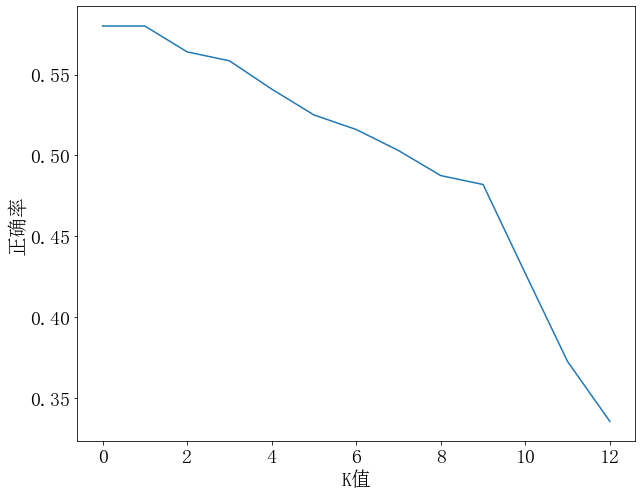
\includegraphics{D:/yy/Documents/GitHub/LaTex-Projects/NLP/hw2/note.figure/不同K值正确率曲线.png}
\caption{img}
\end{figure}

我们发现K越小正确率越高,但是K过小可能发生过拟合,所以最后选取了K=4

\begin{verbatim}
K为4时,平均正确率较高55.85%
第  1 组类别,正确率: 0.43
第  2 组类别,正确率: 0.55
第  3 组类别,正确率: 0.51
第  4 组类别,正确率: 0.38
第  5 组类别,正确率: 0.56
第  6 组类别,正确率: 0.44
第  7 组类别,正确率: 0.42
第  8 组类别,正确率: 0.46
第  9 组类别,正确率: 0.67
第 10 组类别,正确率: 0.57
第 11 组类别,正确率: 0.70
第 12 组类别,正确率: 0.62
第 13 组类别,正确率: 0.51
第 14 组类别,正确率: 0.57
第 15 组类别,正确率: 0.57
第 16 组类别,正确率: 0.50
第 17 组类别,正确率: 0.56
第 18 组类别,正确率: 0.72
第 19 组类别,正确率: 0.43
第 20 组类别,正确率: 0.65
\end{verbatim}

\hypertarget{ux524dux9988ux578bux795eux7ecfux7f51ux7edc}{%
\subsubsection{前馈型神经网络}\label{ux524dux9988ux578bux795eux7ecfux7f51ux7edc}}

使用tensorflow神经网络框架

\begin{Shaded}
\begin{Highlighting}[]
\ImportTok{import}\NormalTok{ tensorflow }\ImportTok{as}\NormalTok{ tf}
\ImportTok{import}\NormalTok{ tensorflow.keras }\ImportTok{as}\NormalTok{ keras}
\ImportTok{import}\NormalTok{ tensorflow.keras.layers }\ImportTok{as}\NormalTok{ layers}
\end{Highlighting}
\end{Shaded}

构造训练集,并随机打乱,设置batch大小为16,重复原始数据集5次,得到包含
\(17835*5=89175\)
个元素的数据集,每次对其进行训练(原始数据集太小了,放大了5倍)

\begin{Shaded}
\begin{Highlighting}[]
\NormalTok{train\_x, train\_y }\OperatorTok{=}\NormalTok{ [], []}
\NormalTok{test\_x, test\_y }\OperatorTok{=}\NormalTok{ [], []}
\NormalTok{tmp }\OperatorTok{=}\NormalTok{ [w }\ControlFlowTok{for}\NormalTok{ words }\KeywordTok{in}\NormalTok{ test\_words }\ControlFlowTok{for}\NormalTok{ w  }\KeywordTok{in}\NormalTok{ words]}
\ControlFlowTok{for}\NormalTok{ i }\KeywordTok{in} \BuiltInTok{range}\NormalTok{(}\DecValTok{20}\NormalTok{):}
    \ControlFlowTok{for}\NormalTok{ w }\KeywordTok{in}\NormalTok{ test\_words[i]:  }\CommentTok{\# 测试集}
\NormalTok{        x }\OperatorTok{=}\NormalTok{ word2vector(w)}
\NormalTok{        test\_x.append(x)}
\NormalTok{        test\_y.append(i)}
    \ControlFlowTok{for}\NormalTok{ w }\KeywordTok{in}\NormalTok{ words[i]:  }\CommentTok{\# 训练集}
        \ControlFlowTok{if}\NormalTok{ w }\KeywordTok{not} \KeywordTok{in}\NormalTok{ tmp:  }\CommentTok{\# 训练集元素不能在测试集中出现}
\NormalTok{            x }\OperatorTok{=}\NormalTok{ word2vector(w)}
\NormalTok{            train\_x.append(x)}
\NormalTok{            train\_y.append(i)}
\CommentTok{\# 转化为np.ndarray的形式}
\NormalTok{train\_x }\OperatorTok{=}\NormalTok{ np.array(train\_x)}
\NormalTok{train\_y }\OperatorTok{=}\NormalTok{ np.array(train\_y)}
\NormalTok{test\_x }\OperatorTok{=}\NormalTok{ np.array(test\_x)}
\NormalTok{test\_y }\OperatorTok{=}\NormalTok{ np.array(test\_y)}
\CommentTok{\# 构建为tf.data.Dataset数据类型}
\NormalTok{train }\OperatorTok{=}\NormalTok{ tf.data.Dataset.from\_tensor\_slices((train\_x, train\_y))}
\NormalTok{train }\OperatorTok{=}\NormalTok{ train.shuffle(}\DecValTok{10000}\NormalTok{).batch(}\DecValTok{16}\NormalTok{).repeat(}\DecValTok{5}\NormalTok{)  }\CommentTok{\# 对数据集进行预处理}
\NormalTok{test }\OperatorTok{=}\NormalTok{ tf.data.Dataset.from\_tensor\_slices((test\_x, test\_y))}
\end{Highlighting}
\end{Shaded}

构建神经网络模型,包含一个含有32个神经元的隐藏层,使用sigmoid作为激活函数,softmax函数作为输出层的激活函数,使用交叉熵损失函数.

\begin{Shaded}
\begin{Highlighting}[]
\NormalTok{model }\OperatorTok{=}\NormalTok{ keras.Sequential([}
\NormalTok{    layers.Dense(}\DecValTok{32}\NormalTok{, activation}\OperatorTok{=}\StringTok{\textquotesingle{}sigmoid\textquotesingle{}}\NormalTok{, input\_shape}\OperatorTok{=}\NormalTok{[N,]),  }\CommentTok{\# 隐藏层}
\NormalTok{    layers.Dense(}\DecValTok{20}\NormalTok{, activation}\OperatorTok{=}\StringTok{\textquotesingle{}softmax\textquotesingle{}}\NormalTok{)  }\CommentTok{\# 输出层}
\NormalTok{])}
\NormalTok{model.}\BuiltInTok{compile}\NormalTok{(optimizer}\OperatorTok{=}\StringTok{\textquotesingle{}adam\textquotesingle{}}\NormalTok{,  }\CommentTok{\# 优化器}
\NormalTok{             loss }\OperatorTok{=}\NormalTok{ keras.losses.SparseCategoricalCrossentropy(),  }\CommentTok{\# 损失函数}
\NormalTok{             metrics}\OperatorTok{=}\NormalTok{[}\StringTok{\textquotesingle{}accuracy\textquotesingle{}}\NormalTok{])  }\CommentTok{\# 将准确率作为预测指标}
\NormalTok{history }\OperatorTok{=}\NormalTok{ model.fit(train, epochs}\OperatorTok{=}\DecValTok{20}\NormalTok{, validation\_data}\OperatorTok{=}\NormalTok{(test\_x, test\_y))}
\end{Highlighting}
\end{Shaded}

训练20次,得到的损失和准确率如图下图所示,15次以后,验证集准确率基本稳定在70\%,训练集准确率稳定在80\%左右.
下图准确率最终稳定在 70.9\%

\begin{figure}
\centering
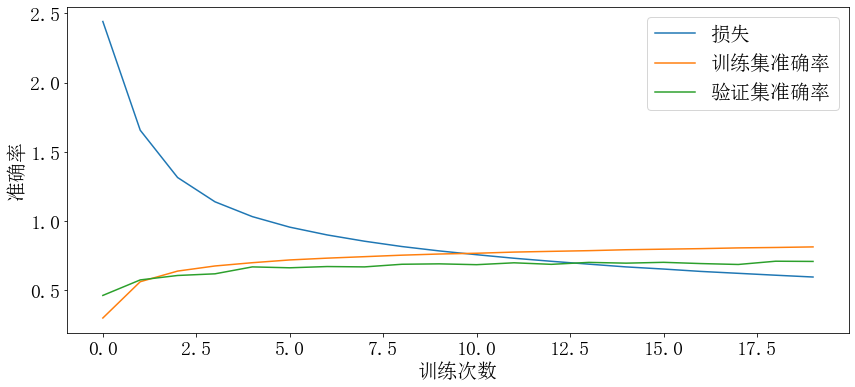
\includegraphics{D:/yy/Documents/GitHub/LaTex-Projects/NLP/hw2/note.figure/神经网络训练过程.png}
\caption{}
\end{figure}

神经网络日志如下:

\begin{verbatim}
Epoch 1/20
5575/5575 [==============================] - 18s 3ms/step - loss: 2.4416 - accuracy: 0.3004 - val_loss: 2.0228 - val_accuracy: 0.4635
Epoch 2/20
5575/5575 [==============================] - 19s 3ms/step - loss: 1.6565 - accuracy: 0.5624 - val_loss: 1.5213 - val_accuracy: 0.5755
Epoch 3/20
5575/5575 [==============================] - 17s 3ms/step - loss: 1.3149 - accuracy: 0.6392 - val_loss: 1.3432 - val_accuracy: 0.6075
Epoch 4/20
5575/5575 [==============================] - 19s 3ms/step - loss: 1.1396 - accuracy: 0.6762 - val_loss: 1.2247 - val_accuracy: 0.6195
Epoch 5/20
5575/5575 [==============================] - 16s 3ms/step - loss: 1.0325 - accuracy: 0.6998 - val_loss: 1.1397 - val_accuracy: 0.6695
Epoch 6/20
5575/5575 [==============================] - 16s 3ms/step - loss: 0.9565 - accuracy: 0.7197 - val_loss: 1.0940 - val_accuracy: 0.6630
Epoch 7/20
5575/5575 [==============================] - 16s 3ms/step - loss: 0.9004 - accuracy: 0.7326 - val_loss: 1.0728 - val_accuracy: 0.6720
Epoch 8/20
5575/5575 [==============================] - 21s 4ms/step - loss: 0.8550 - accuracy: 0.7433 - val_loss: 1.0415 - val_accuracy: 0.6695
Epoch 9/20
5575/5575 [==============================] - 21s 4ms/step - loss: 0.8165 - accuracy: 0.7541 - val_loss: 1.0145 - val_accuracy: 0.6885
Epoch 10/20
5575/5575 [==============================] - 25s 5ms/step - loss: 0.7849 - accuracy: 0.7625 - val_loss: 1.0055 - val_accuracy: 0.6915
Epoch 11/20
5575/5575 [==============================] - 29s 5ms/step - loss: 0.7575 - accuracy: 0.7680 - val_loss: 1.0040 - val_accuracy: 0.6855
Epoch 12/20
5575/5575 [==============================] - 27s 5ms/step - loss: 0.7320 - accuracy: 0.7765 - val_loss: 0.9934 - val_accuracy: 0.6990
Epoch 13/20
5575/5575 [==============================] - 27s 5ms/step - loss: 0.7100 - accuracy: 0.7818 - val_loss: 1.0070 - val_accuracy: 0.6880
Epoch 14/20
5575/5575 [==============================] - 29s 5ms/step - loss: 0.6894 - accuracy: 0.7867 - val_loss: 0.9691 - val_accuracy: 0.7020
Epoch 15/20
5575/5575 [==============================] - 26s 5ms/step - loss: 0.6694 - accuracy: 0.7934 - val_loss: 0.9863 - val_accuracy: 0.6965
Epoch 16/20
5575/5575 [==============================] - 25s 5ms/step - loss: 0.6540 - accuracy: 0.7975 - val_loss: 0.9796 - val_accuracy: 0.7025
Epoch 17/20
5575/5575 [==============================] - 26s 5ms/step - loss: 0.6368 - accuracy: 0.8013 - val_loss: 0.9810 - val_accuracy: 0.6935
Epoch 18/20
5575/5575 [==============================] - 25s 4ms/step - loss: 0.6231 - accuracy: 0.8067 - val_loss: 1.0227 - val_accuracy: 0.6870
Epoch 19/20
5575/5575 [==============================] - 25s 5ms/step - loss: 0.6094 - accuracy: 0.8097 - val_loss: 0.9688 - val_accuracy: 0.7105
Epoch 20/20
5575/5575 [==============================] - 24s 4ms/step - loss: 0.5964 - accuracy: 0.8138 - val_loss: 0.9776 - val_accuracy: 0.7090
\end{verbatim}

\hypertarget{ux603bux7ed3}{%
\subsection{总结}\label{ux603bux7ed3}}

通过本次实验,学会了使用 \texttt{nltp}
包对文档进行分词操作,对原式文档进行预处理,使用KNN和前馈神经网络两种不同的模型对文档进行分类预测,正确率分别在55.85\%和70.9\%左右,效果均不是非常好,仍有待改进.

\end{document}
